The project planification can be broken down to four main phases: those of Analysis, Documentation \& Specification, Development \& Testing, and the MVP. Following is a more detailed explanation of each one:

\section{Analysis}
The main part of this work will be completed during the GEP Course. This includes the definition of the goal and scope of the project itself, as well as the time planning, economic and environmental studies and presentation of the project. Non-technical documentation is assumed as one of the outputs of this phase, which will span across the first two sprints.

\section{Documentation \& Specification}
During this phase, the design, specification and resulting documentation will be delivered. The documentation will be of a technical nature and consist of three main parts:

\begin{itemize}
\item Use cases, or Functional documentation, which defines the products from a usage point of view: what the product will be able to do, and what it will allow a user to achieve. The expected output of this part, therefore, is a document that will specify the use cases and functional requirements of the designed solution.

\item Architecture design, which defines the product from a technical point of view. This will include the design patterns that will be applied with the justification of their usage, alongside with a diagram of the architecture for a more clear understanding. The expected output of this part is a technical document that describes the architectural design of the solution.

\item User documentation. A user-oriented set of instructions and descriptions meant to make the use of the designed product possible and easy. The expected output of this part is a comprehensive and highly available document describing the features of the designed product and how to use them.
\end{itemize}

This phase will span across sprints 3 and 4 mainly, except for the user documentation part, which will be produced in a coordinated manner alongside the Development phase.

\section{Development \& Testing}
This phase consists of the actual implementation of the solution. It can be also broken down to three main parts:

\begin{itemize}
\item Testing: Against what could seem more intuitive, this can be considered the first part of this phase, as the development will be oriented according to the TDD paradigm. The first step, therefore, is to have a suitable test environment, platform and strategy upon which to carry out the development.

\item Development: This part consists in actually implementing the designed solution and includes, as a first step, the setting up of a local development environment. Also, as per the reasons exposed during the description of the previous part, it will be closely entwined with the testing, so these two first parts will be carried out in a parallel manner. This means that, because of the TDD paradigm, there will be a workload of testing previous to any coding work. Furthermore, as noted before, during this stage it is highly probable that some of the workload will be dedicated to the user documentation, for several reasons: on the one hand, unexpected changes that may arise, and on the other hand, some documentation tools or frameworks may be used to generate said documentation. Usually these tools are used during development time and have presence in the source code itself.

\item Deployment: Once the designed product is implemented and the business logic is correctly working, the next part will be to design and implement an easy process to deploy and make the solution production-ready as easily as possible. Although also implies testing and development like in the previous steps, it can conceptually be considered an altogether different goal. The output of this part includes two aspects: on the one hand, the deployment infrastructure and process itself, and on the other hand, having the solution working in a production environment.
\end{itemize}

This phase will span across sprints 5 and 6 for the testing and development parts, and will use sprint 7 for the implementation of deployment infrastructure.

\section{Consumer MVP}
This final phase has the only goal of providing a proof-of-concept for the whole solution. Since the goal of the product is to provide an easy-to-use solution to be consumed by custom solutions, the output of this phase will be a quick-and-dirty solution that will use the product deployed during sprint 7 and provide an hypothetical profit. This demo will be built during sprint 8. The expected output of this sprint will be a simple client application.

\section{Gantt diagram}
Following is the Gantt diagram outlining the different project phases (Figure \ref{fig:ganttdiagram}) along with a detailed breakdown (Figure \ref{fig:ganttdetail})

\begin{figure}
	\centering
		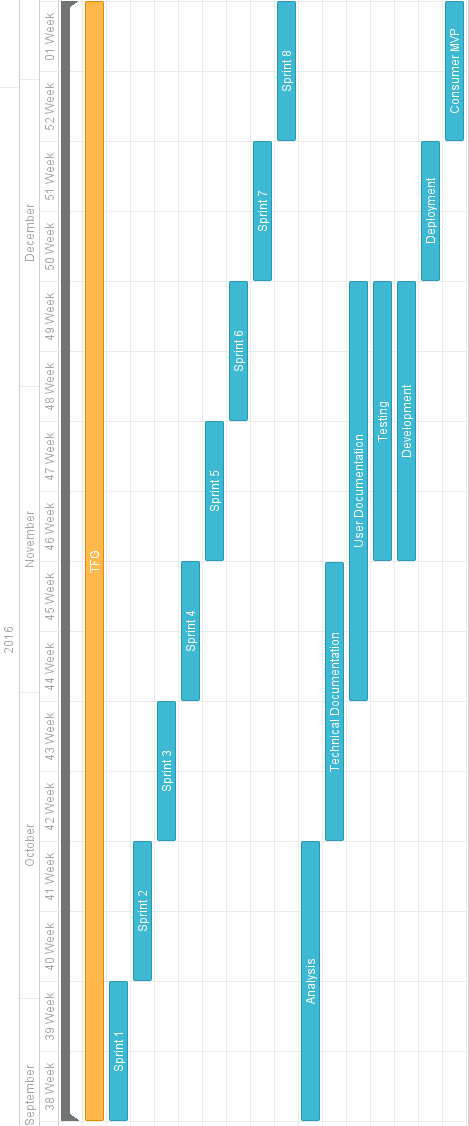
\includegraphics[scale=0.4]{g1.png}
	\caption{Gantt Diagram}
	\label{fig:ganttdiagram}
\end{figure}

\begin{figure}
	\centering
		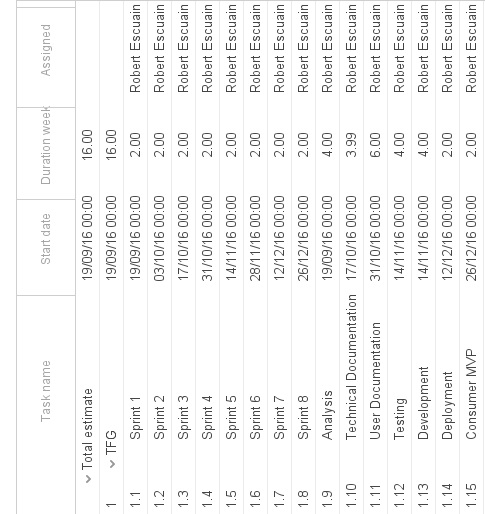
\includegraphics[scale=0.5]{g2.png}
	\caption{Gantt Detail}
	\label{fig:ganttdetail}
\end{figure}